\chapter{Une architecture d'habitats intelligents modernisée}
\label{chap:5}

\section{Introduction}

Il a été vu, dans les chapitres précédents qu'au fil des ans, diverses architectures de maisons intelligentes ont été proposées et mises en place au sein de laboratoires ou dans de réelles habitations pour mener des activités de recherche \citep{DJCook2003,Helal2005,Giroux2009,Cook2013,Bouchard2014,Lago2017,Plantevin2018}. Ces travaux se sont particulièrement intéressés à l'utilisation de capteurs, d'effecteurs et de techniques d'apprentissage machine pour la mise en application de l'\acl{IAm} comme méthode empirique afin de soutenir l'autonomie des personnes âgées et le suivi de la santé. Cependant, bien que chacun de ces travaux se distingue des autres, tous proposent différentes méthodes pour résoudre le problème principal qu'il cherchent à résoudre demeure la reconnaissance d'activités. Les avantages et les inconvénients de chaque architecture d'habitats intelligents ont déjà été discutés dans cette thèse et le principal problème qui a été identifié réside dans le manque de fiabilité et l'évolutivité de ces implémentations. En effet, la plupart des architectures admettent au moins un point de défaillance unique (\acl{SPOF} ou \acs{SPOF}) principalement à cause de leur implémentation centralisée, ou \og monolithique \fg. Néanmoins, il a aussi été montré que \cite{Plantevin2018} ont adressé cette problématique en introduisant un nouveau type d'architecture basée sur l'utilisation de transducteurs intelligents distribués. Cependant, bien que cette implémentation ait été pensée pour être une architecture de maisons intelligentes prête à l'emploi en situation réelle d'utilisation, sa conception ne semble pas suffisamment adaptée aux environnements de recherche. En effet, la simplicité de mise en place de nouvelles méthodes pour la reconnaissance d'activités et de nouveaux protocoles expérimentaux semble avoir été oubliés dans cette implémentation.

Par ailleurs, dans la comparaison des différentes architectures de maisons intelligentes proposées au chapitre \ref{chap:2}, le principal inconvénient des solutions existantes qui a été identifié concerne leur manque de flexibilité quant à l'intégration de nouveaux matériels et plus spécifiquement, les \textit{wearable devices}. En effet, pour réaliser la reconnaissance d'activités, la plupart des méthodes proposées avec ses dispositifs sont des applications complètes. La plupart du temps, les différents processus qui composent la reconnaissance sont encapsulés au sein d'un unique composant logiciel immuable. Il devient donc difficile de les modifier. De plus, le fait de disposer d'une unique application ne favorise pas la réutilisation de certains mécanismes communs à plusieurs méthodes. Ceux-ci doivent donc généralement être soit développés à nouveau, soit adaptés afin de pouvoir supporter des modifications dans la méthode proposée. De plus, l'exploitation de ce genre d'application \og prête à l'emploi \fg est, la plupart du temps, complexifiée. En effet, selon les dépendances, le langage de programmation et la plateforme, elles peuvent être difficiles à adapter et à déployer d'un environnement à un autre (\textit{p. ex.} entre deux laboratoires de recherche différents).

Ainsi, ce travail présente un autre type d'architecture de maisons intelligentes qui se veut fiable et évolutive dont l'implémentation est inspirée des architectures de \textit{cloud} privées sur site. Cette architecture vise à résoudre la plupart des problèmes identifiés au sein des implémentations précédemment proposées sans qu'il soit nécessaire de remplacer leur structure au complet. En effet, l'implémentation présentée dans ce chapitre a été pensée pour à la fois être déployée en l'état, ou pour s'intégrer aux architectures existantes, remplaçant ainsi les entités centrales des architectures monolithiques. L'objectif principal de cette implémentation est alors de pouvoir y déployer facilement de nouveaux composants logiciels expérimentaux indépendamment des différences dans leur conception, tant en termes de langages de programmation que de librairies requises ou de plateforme supportées. Ceci dans le but de favoriser l'interopérabilité entre les différents processus, leur réutilisation ainsi que leur mise à l'échelle vis-à-vis de la quantité de ressources requise.

La suite de ce chapitre comporte une première section qui présente en détail l'architecture d'habitats intelligents proposée. Ensuite, les expérimentations sont décrites dans une seconde section. De plus, cette section propose une discussion des observations réalisées. Finalement, dans une dernière partie, une conclusion est dressée quant à ce second travail.

\section{Architecture Proposée}

L'architecture introduite dans ce chapitre a été conçue pour être compatible avec la majorité des architectures de maisons intelligentes présentes dans la littérature. Par conséquent, celle-ci peut être considérée comme une extension du travail proposé par \cite{Plantevin2018}, puisqu'ils ont concentré leurs efforts sur la suppression des \acsp{SPOF} dans le but d'améliorer la fiabilité globale des habitats intelligents existants. Néanmoins, l'idée principale de ce travail est d'aller plus loin dans l'idée de rendre ces architectures plus fiables et plus flexibles. Pour ce faire, ce chapitre présente une implémentation qui repose sur l'utilisation des microservices plutôt qu'une approche monolithique.

\subsection{Microservices}

Les architectures de microservices sont récemment apparues comme un nouveau paradigme pour la programmation d'applications et dont l'origine se base sur le concept d'\ac{AOS} \citep{MacKenzie2006}. Comme le montre la figure \ref{fig:mono_micro}, cette approche suggère de diviser une application en un ensemble de services plus petits, indépendants et interconnectés. En comparaison aux applications monolithiques, où tous les composants logiciels se trouvent dans une seule instance, les services exécutent des fonctions plus détaillées et précises. Bien que les architectures monolithiques soient simples à implémenter, les architectures de microservices présentent, elles aussi, différents avantages. La première concerne l'\emph{agilité} des microservices. En effet, puisque les applications sont fragmentées au niveau le plus élémentaire de leurs fonctionnalités, chaque service devient individuellement plus facile à maintenir et beaucoup plus rapide à développer et à déployer. Le second avantage principal demeure la \emph{réutilisabilité}. Les microservices permettent aux développeurs de créer des applications en utilisant certains fragments déjà existants. De plus, la barrière entre les technologies (\textit{p. ex.} les langages de programmation) est réduite puisque les services fonctionnent de manière indépendante. En ce sens, cet \emph{agnosticisme technologique} permet d'obtenir des applications hétérogènes du point de vue des technologies dans leur conception. Par ailleurs, un autre avantage offert par les architectures de microservices concerne la mise à l'échelle des différents composants à mesure que la demande pour une application augmente. En cas de forte demande ponctuelle, il est possible soit d'augmenter la quantité de ressources allouées, soit d'augmenter le nombre d'instances pour les services les plus impactés, plutôt que pour l'intégralité de application. Il s'agit respectivement de l'\emph{extensibilité dynamique horizontale} et de l'\emph{extensibilité dynamique verticale}. Enfin, puisque les composants d'une application dans une architecture de microservices sont généralement distribués, l'application est en mesure de supporter les pannes au niveau des services qui la composent. En effet, lorsqu'un service est en panne, la fonctionnalité dont il est responsable devient inopérante, mais le fonctionnement du reste de l'application n'est pas altéré. De plus, il est possible de mettre en place différents mécanismes pour remédier aux défaillances inattendues afin d'augmenter la résilience et la \emph{fiabilité} de l'ensemble du système.

\begin{figure}[t]
	\centering
	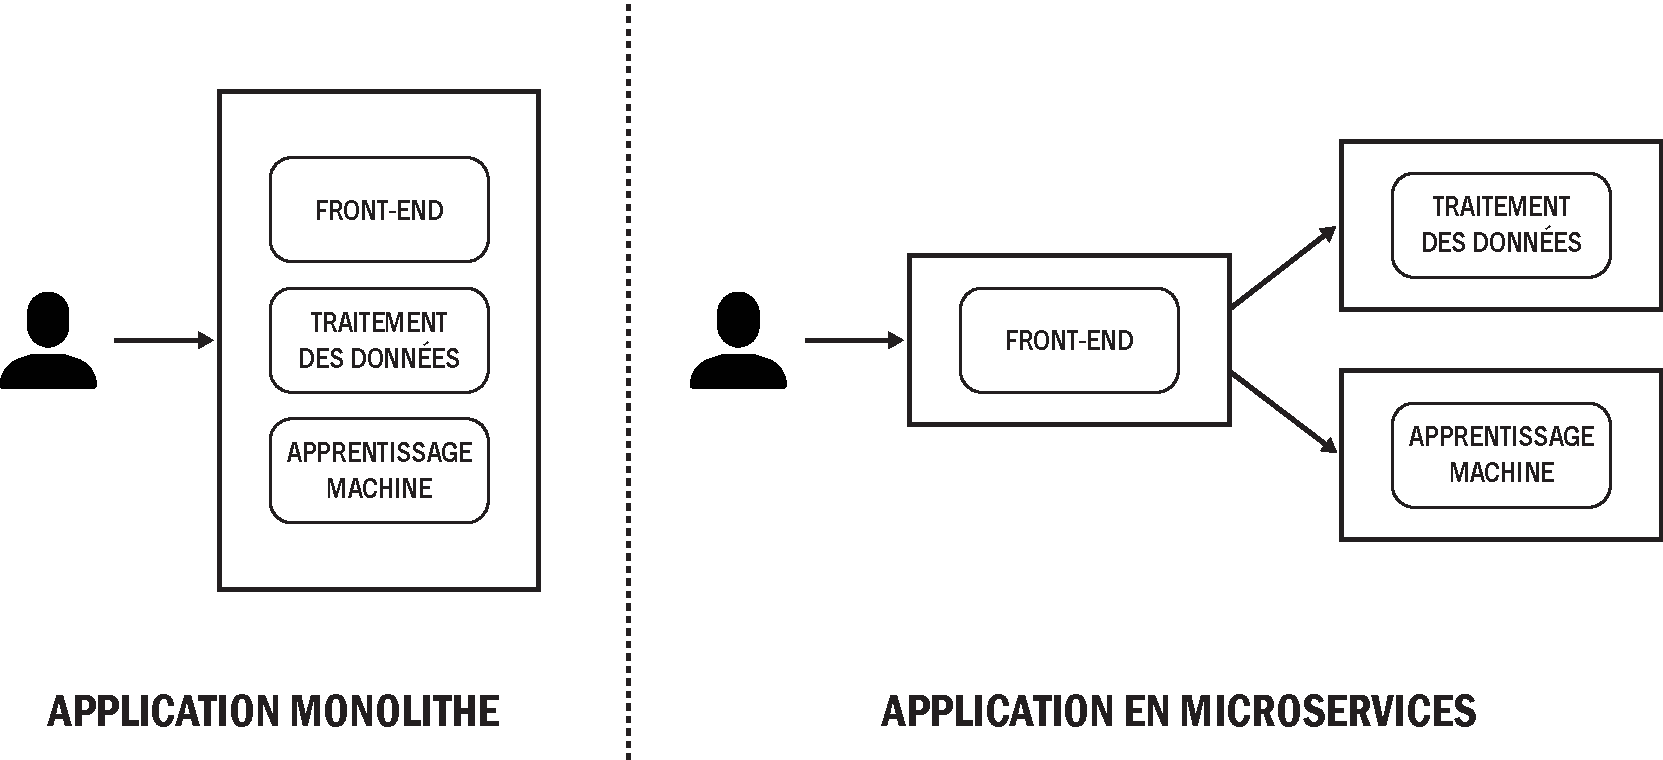
\includegraphics[width=.8\linewidth]{chapter5/mono_micro.pdf}
		\caption{Comparaison entre les architectures monolithiques et de microservices selon un exemple d'application qui vise à résoudre un problème d'apprentissage machine par le biais d'une interface graphique.}
	\label{fig:mono_micro}
\end{figure}

\begin{figure}[hb!]
	\centering
	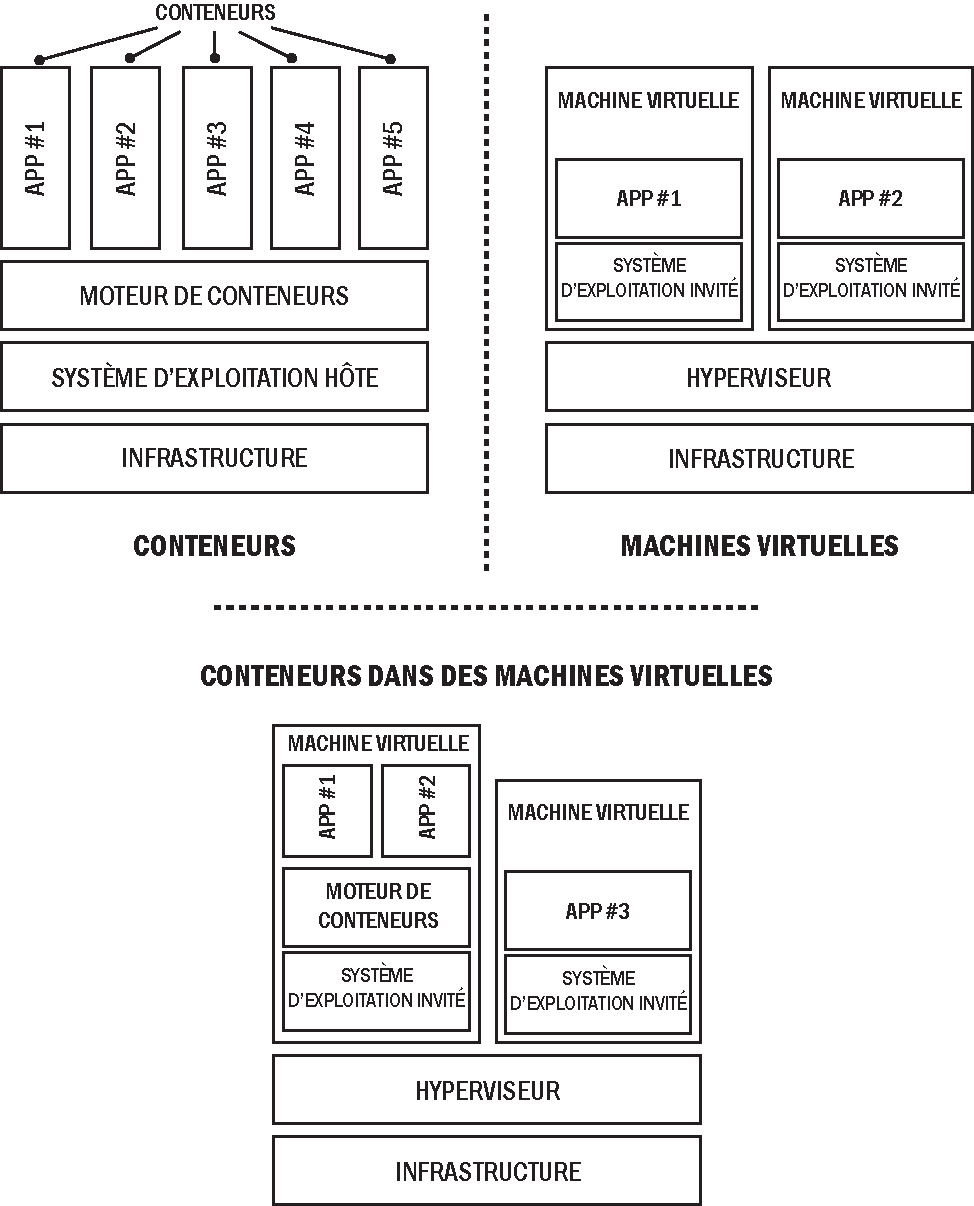
\includegraphics[width=.8\linewidth]{chapter5/containers_vms.pdf}
		\caption{Illustration détaillée des trois principales techniques de virtualisation pour la mise en place d'une architecture de microservices.}
	\label{fig:containers_vms}
\end{figure}

Actuellement, il existe de nombreuses façons de mettre en place une architecture de microservices, la plus courante étant l'utilisation d'outils de virtualisation tels que les machines virtuelles (\acsp{VM}) traditionnelles, les conteneurs ou les conteneurs à l'intérieur de \acsp{VM}. La figure \ref{fig:containers_vms} fournit une représentation graphique de ces trois différentes implémentations. Même si le choix de la méthode de virtualisation n'affecte pas les possibilités offertes par les architectures de microservices, il existe des différences significatives entre l'utilisation de \acsp{VM} traditionnelles et les conteneurs qu'il semble important de détailler. La principale différence réside dans le fait que les conteneurs proposent une virtualisation au niveau du système d'exploitation alors que les \acsp{VM} offrent une virtualisation au niveau du matériel. En ce qui concerne les \acsp{VM}, l'hyperviseur permet de cloisonner des portions du matériel. En effet, son rôle est d'attribuer à chaque machine virtuelle les ressources nécessaires en fonction des ressources physiques du système hôte. De manière générale, il existe deux types d'hyperviseurs. Dans un premier temps, il y a les hyperviseurs de système natif qui s'exécutent directement sur le matériel du système hôte. En ce sens, ceux-ci prennent la place du système d'exploitation de l'hôte et planifient directement l'utilisation des ressources allouées aux machines virtuelles en fonction du matériel. Dans un second temps, les hyperviseurs hébergés fonctionnent comme une couche logicielle supplémentaire au sein du système d'exploitation hôte. Ainsi, ils permettent de dissocier les systèmes d'exploitation invités (virtualisés) du système d'exploitation hôte.

Alternativement, les conteneurs permettent aux instances virtuelles de partager un système d'exploitation hôte unique. Par conséquent, puisque les conteneurs n'ont pas à embarquer un système d'exploitation, les images virtualisées demeurent beaucoup plus légères que celles des \acsp{VM} traditionnelles. De plus, les conteneurs sont, au même titre que les \acsp{VM}, isolés du système hôte, c'est-à-dire, qu'ils s'exécutent dans des espaces séparés à la fois les uns des autres, mais également de certaines parties du système d'exploitation hôte. Une telle isolation permet donc une utilisation plus efficace des ressources. Enfin, les conteneurs sont très rapides à créer et à détruire puisqu'il n'est pas nécessaire de démarrer ou d'arrêter un système d'exploitation à chaque fois. En effet, les conteneurs s'occupent uniquement de compléter le processus dont ils sont en charge.

En somme, une \acs{VM} est une émulation d'un système informatique tandis que les conteneurs sont toutes les unités logiciel qui regroupent le code et toutes ses dépendances requises (\textit{p. ex.} les librairies ou les binaires) qui composent une application. De ce fait, celle-ci peut s'exécuter de façon fiable et rapide d'un environnement à un autre. Ces deux technologies ne sont pas incompatibles puisqu'il est possible de les utiliser ensemble. Cependant, l'exécution de conteneurs à l'intérieur de machines virtuelles est, la plupart du temps, le résultat de l'évolution d'environnements de virtualisation matures déjà existants. Généralement, les conteneurs sont exécutés directement sur le système hôte afin d'optimiser les performances et la latence ou de réduire les coûts des licences des outils de virtualisation et des systèmes d'exploitation.

\subsection{Organisation Matérielle}

\begin{figure}[t]
	\centering
	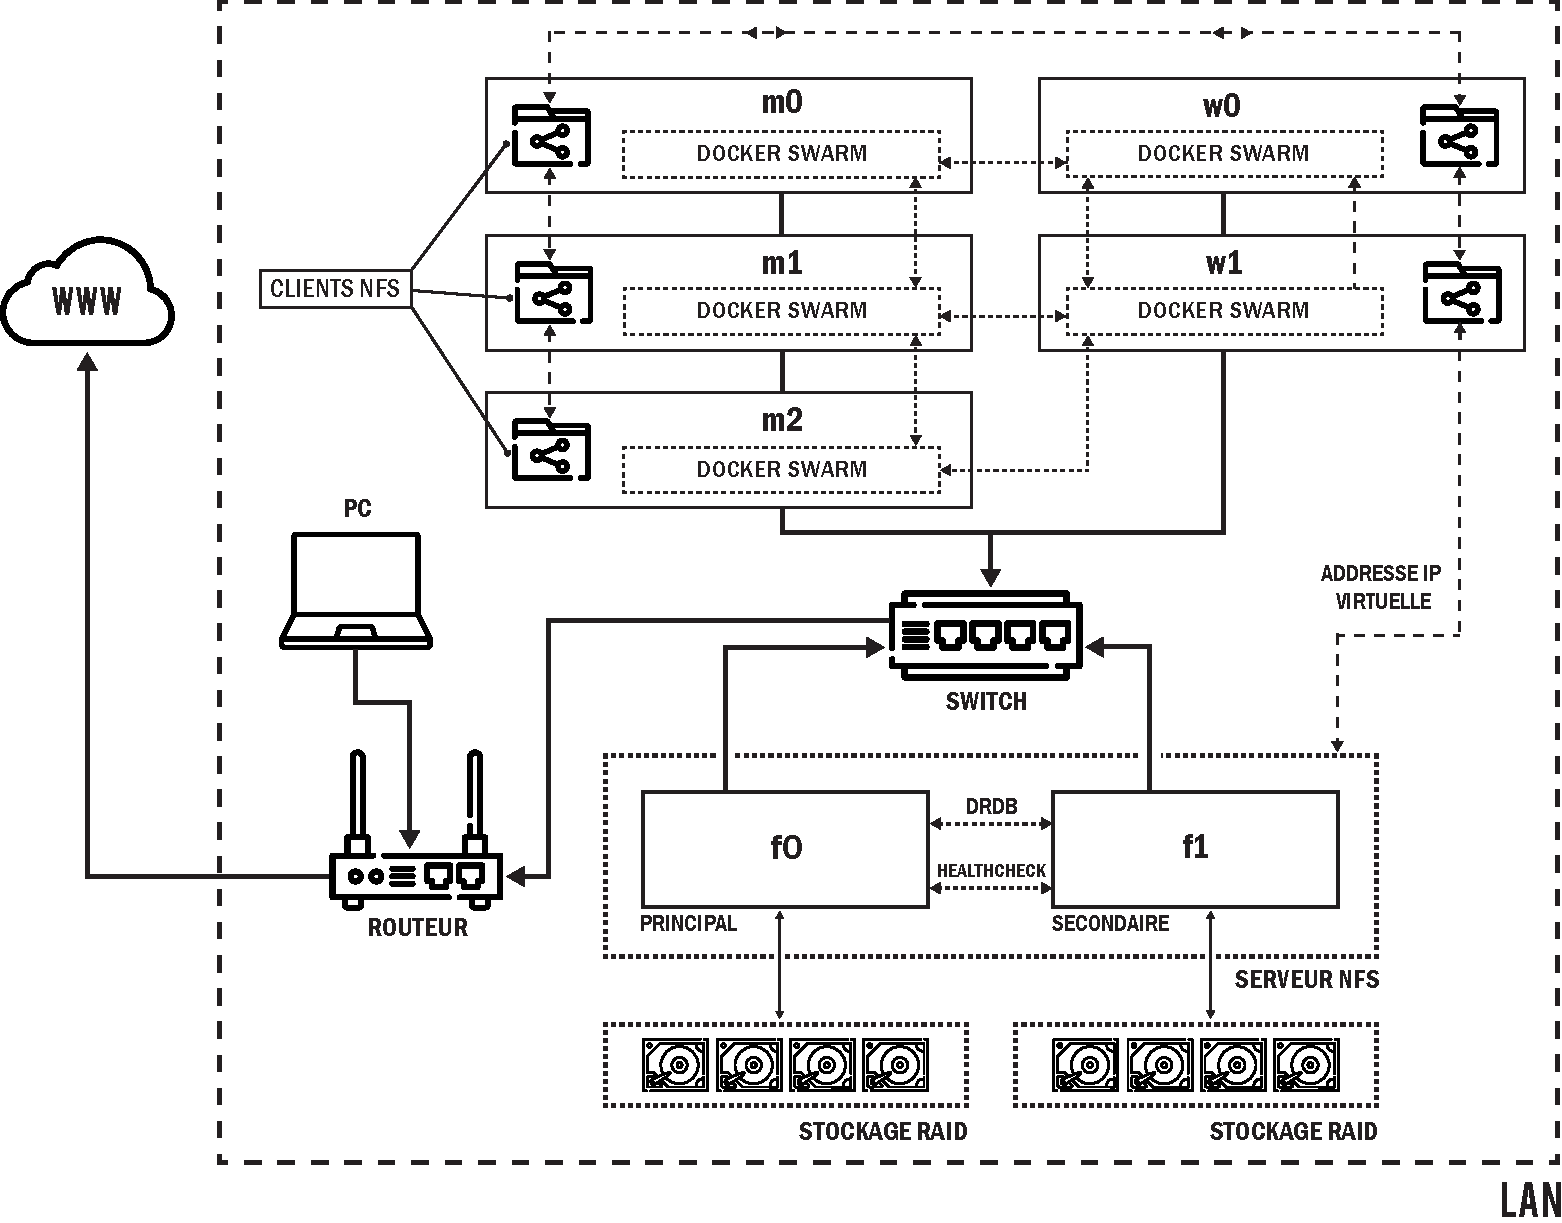
\includegraphics[width=.9\linewidth]{chapter5/proposed_arch.pdf}
        \caption{Organisation matérielle de l'architecture d'habitats intelligents proposée illustrant l'implémentation d'un \textit{cluster} pour le support de l'architecture de microservices ainsi que le système de fichiers distribué.}
	\label{fig:proposed_arch}
\end{figure}

L'organisation matérielle de l'implémentation de l'architecture d'habitats intelligents présentée dans ce chapitre est illustrée par la figure \ref{fig:proposed_arch}. Afin de supporter l'architecture de microservices, cette organisation repose sur un ensemble de cinq n\oe{}uds principaux (\texttt{m0}, \texttt{m1}, \texttt{m2}, \texttt{w0} et \texttt{w1}) qui forment un \textit{cluster} distribué. Par ailleurs, l'implémentation proposée suggère l'utilisation de deux n\oe{}uds supplémentaires (\texttt{f0} et \texttt{f1}) sur chacun desquels une unité de stockage de type \acs{RAID} (\acl{RAID}) est interfacée. L'objectif de ces n\oe{}uds est de fournir un système de fichiers distribué à l'ensemble du \textit{cluster}. En effet, puisque certains conteneurs ont la capacité de monter différents volumes sur le système hôte, un tel système de fichiers offre un moyen fiable de partager des données entre chaque conteneur, quel que soit le n\oe{}ud sur lequel ils s'exécutent. En outre, tous les n\oe{}uds qui composent le \textit{cluster} et le système de fichier distribué sont connectés à un commutateur réseau pour leur permettre de communiquer entre eux. De plus, l'ensemble de l'architecture est isolé à l'intérieur d'un réseau local afin de prévenir les problèmes de sécurité qui pourraient compromettre les expériences et de préserver l'anonymat des participants. Toutefois, pour faciliter la configuration et la maintenance de l'architecture, cette dernière demeure accessible de manière ad hoc avec un ordinateur \textit{via} un routeur qui est, quant a lui, connecté à la fois au Web et au réseau local.

\subsection{Système de fichiers hautement disponible}

Le système de fichiers distribué fourni par les n\oe{}uds \texttt{f0} et \texttt{f1} repose sur le protocole \ac{NFS}. Le principe de ce protocole reste simple, car il est implémenté selon le modèle client/serveur. Un serveur \acs{NFS} gère l'authentification, l'autorisation, l'administration des clients ainsi que les données. Ainsi, une fois autorisés, les clients NFS peuvent accéder aux données distantes de la même manière qu'ils le font localement. En ce sens, chaque n\oe{}ud qui compose le cluster est autorisé à accéder (lecture) et à manipuler les fichiers (création, mise à jour, suppression) de manière classique. Néanmoins, tous les autres n\oe{}uds seront informés des changements qui en résultent.

Cependant, puisque l'idée est de proposer une architecture fiable, le fait de n'avoir qu'un seul serveur \acs{NFS} ne satisfaisait pas cette contrainte. En ce sens, l'outil \acs{DRDB}\footnote{\url{https://www.linbit.com/drbd/}} (\acl{DRDB}) a été mis en place afin que les n\oe{}uds \texttt{f0} et \texttt{f1} puissent proposer un système de fichiers à la fois distribué, mais aussi répliqué. \acs{DRDB} a été paramétré pour effectuer une réplication complète des données stockées entre le serveur principal (\texttt{f0}) et le serveur secondaire (\texttt{f1}), soit le même fonctionnement qu'un système de stockage de type \acs{RAID} 1 en réseau. Afin de favoriser l'intégrité des données plutôt que la vitesse de réplication, la mise en place d'une réplication synchrone constante entre le n\oe{}ud principal et le n\oe{}ud secondaire a été adoptée plutôt qu'une réplication asynchrone ou semi-synchrone. Ainsi, les opérations de manipulation des fichiers réalisées sur le n\oe{}ud principal ne sont considérées comme terminées que lorsque les écritures sur le disque local et sur le disque distant du n\oe{}ud secondaire sont confirmées par ce dernier. Néanmoins, \acs{DRDB} ne fournit aucune fonctionnalité relative à un quelconque mécanisme garantissant la fiabilité du système de fichiers en cas de panne d'un des deux n\oe{}uds. En ce sens, l'outil Heartbeat\footnote{\url{http://www.linux-ha.org/doc/man-pages/re-heartbeat.html}} a également été adopté dans cette implémentation. Cet outil permet de proposer un mécanisme permettant de garantir la haute disponibilité du système de fichiers distribué. En tant que processus d'arrière-plan, le logiciel vise à surveiller l'état des deux serveurs \acs{DRDB}. En cas de défaillance du n\oe{}ud principal (\texttt{f0}), l'adresse \ac{VIP} du système de fichiers distribué pointant vers \texttt{f0} est automatiquement réaffectée au n\oe{}ud secondaire (\texttt{f1}). Ainsi, l'accès aux données n'est en aucun cas compromis lors de la perte d'un seul n\oe{}ud, puisque cette opération est effectuée de manière transparente pour les clients \acs{NFS}.

\subsection{Orchestration des conteneurs}

\begin{figure}[H]
	\centering
	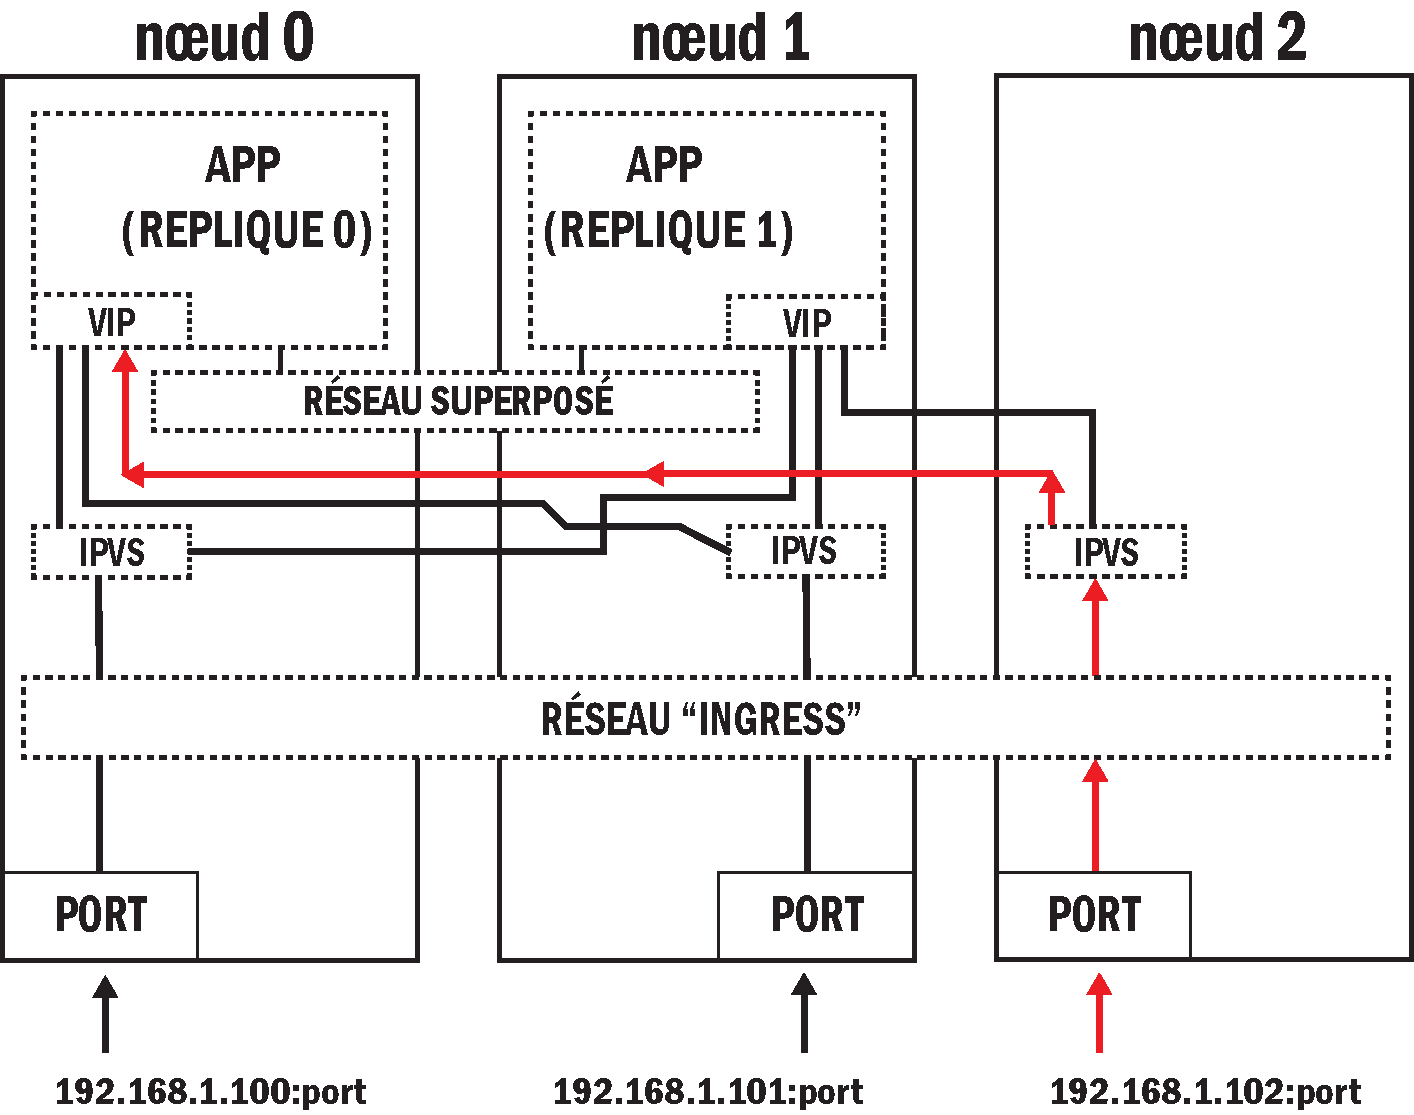
\includegraphics[width=.8\linewidth]{chapter5/swarm_load_balancing.pdf}
        \caption{caption}
	\label{fig:swarm_load_balancing}
\end{figure}

\subsection{Proxy inverse}

\begin{figure}[H]
	\centering
	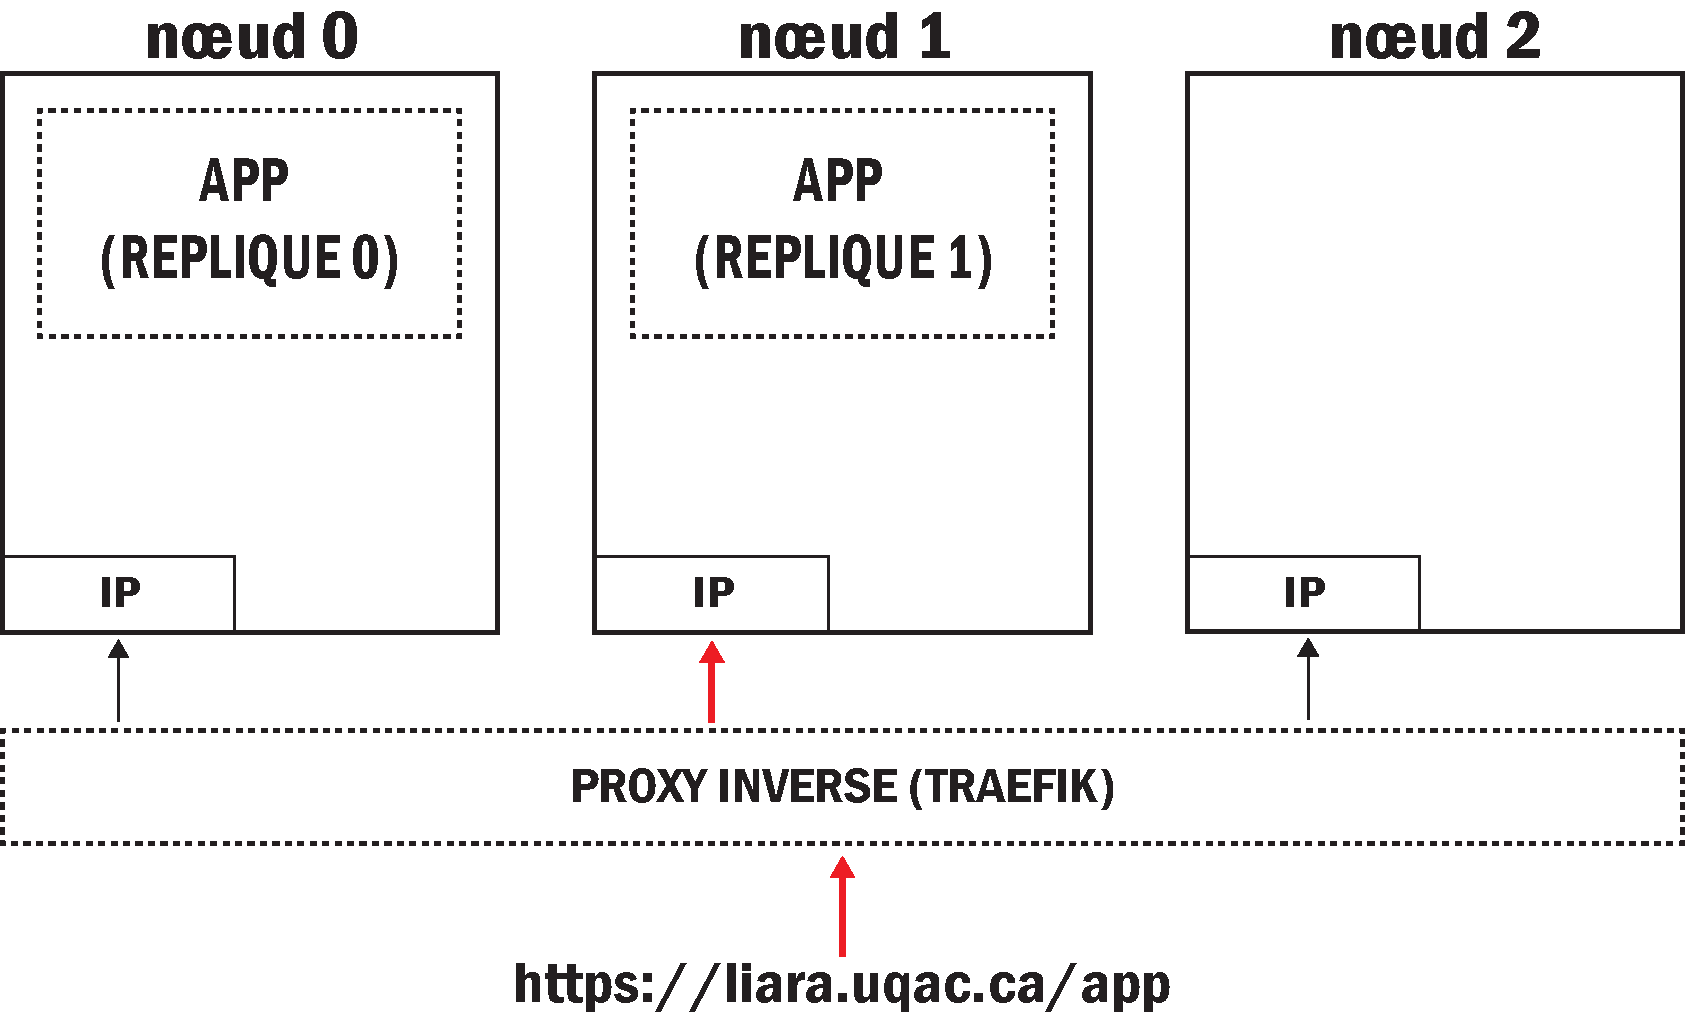
\includegraphics[width=.8\linewidth]{chapter5/arch_reverse_proxy.pdf}
        \caption{caption}
	\label{fig:arch_reverse_proxy}
\end{figure}

\subsection{Gestion du cluster}

\subsection{Base de données répliquée}

\begin{figure}[H]
	\centering
	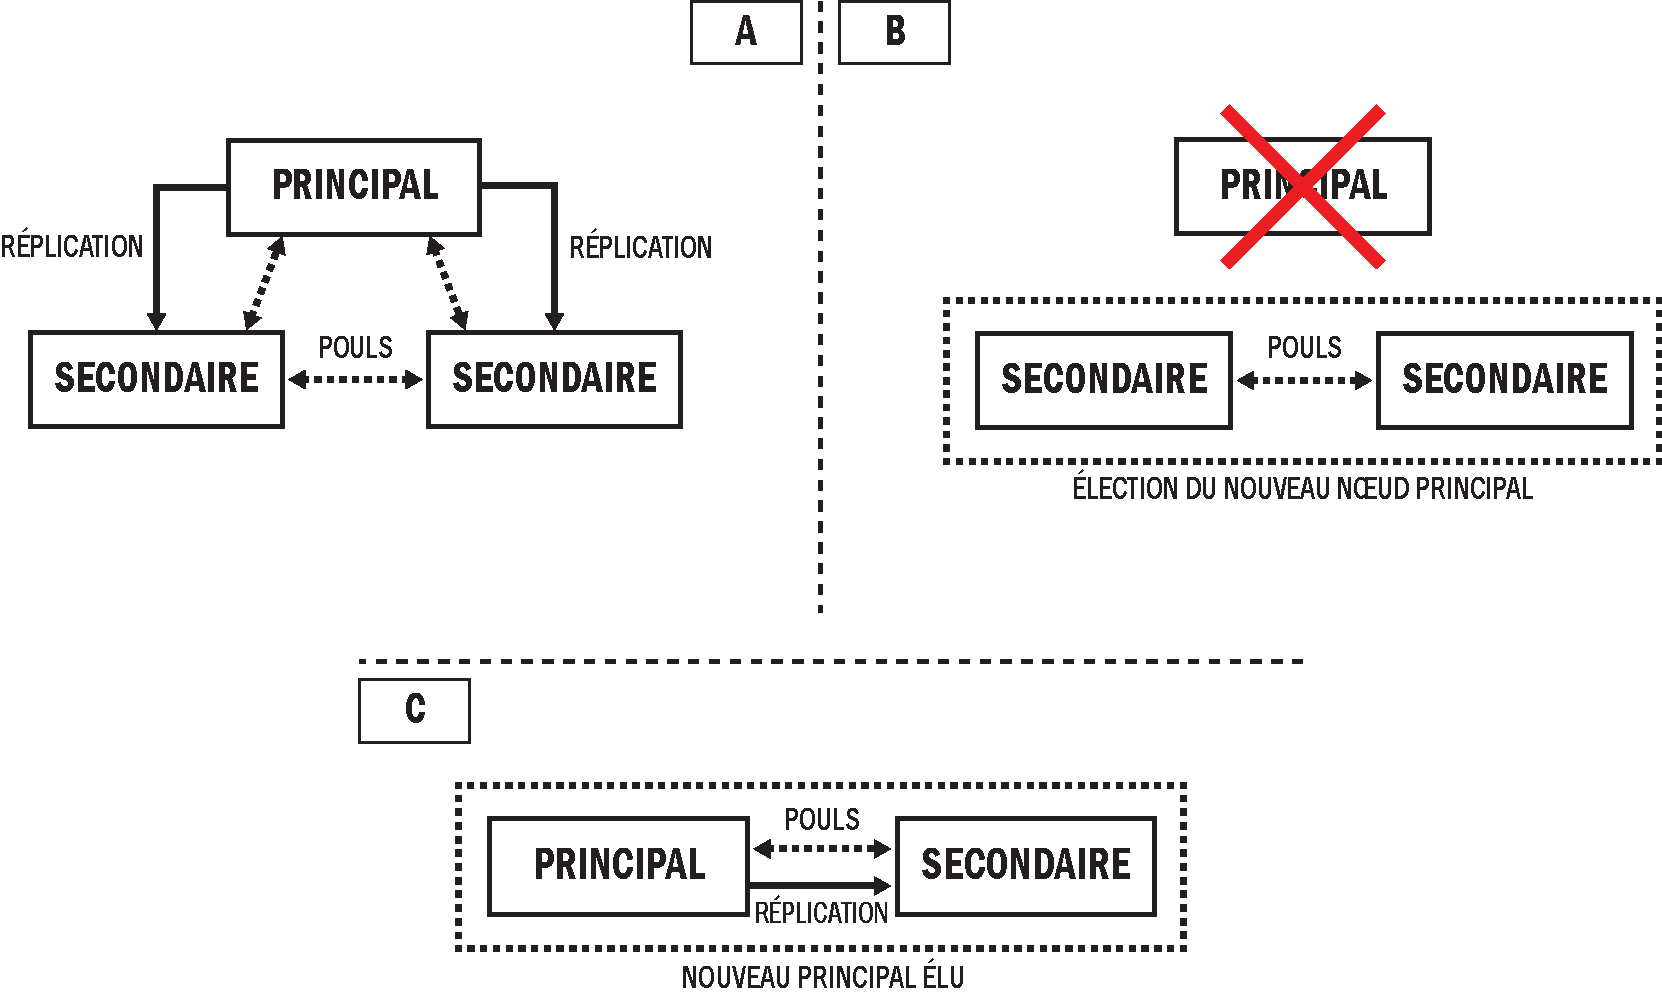
\includegraphics[width=.9\linewidth]{chapter5/mongodb_replication.pdf}
        \caption{caption}
	\label{fig:mongodb_replication}
\end{figure}

\subsection{Dépôt de conteneurs}

\subsection{Organisation des conteneurs}

\begin{figure}[H]
	\centering
	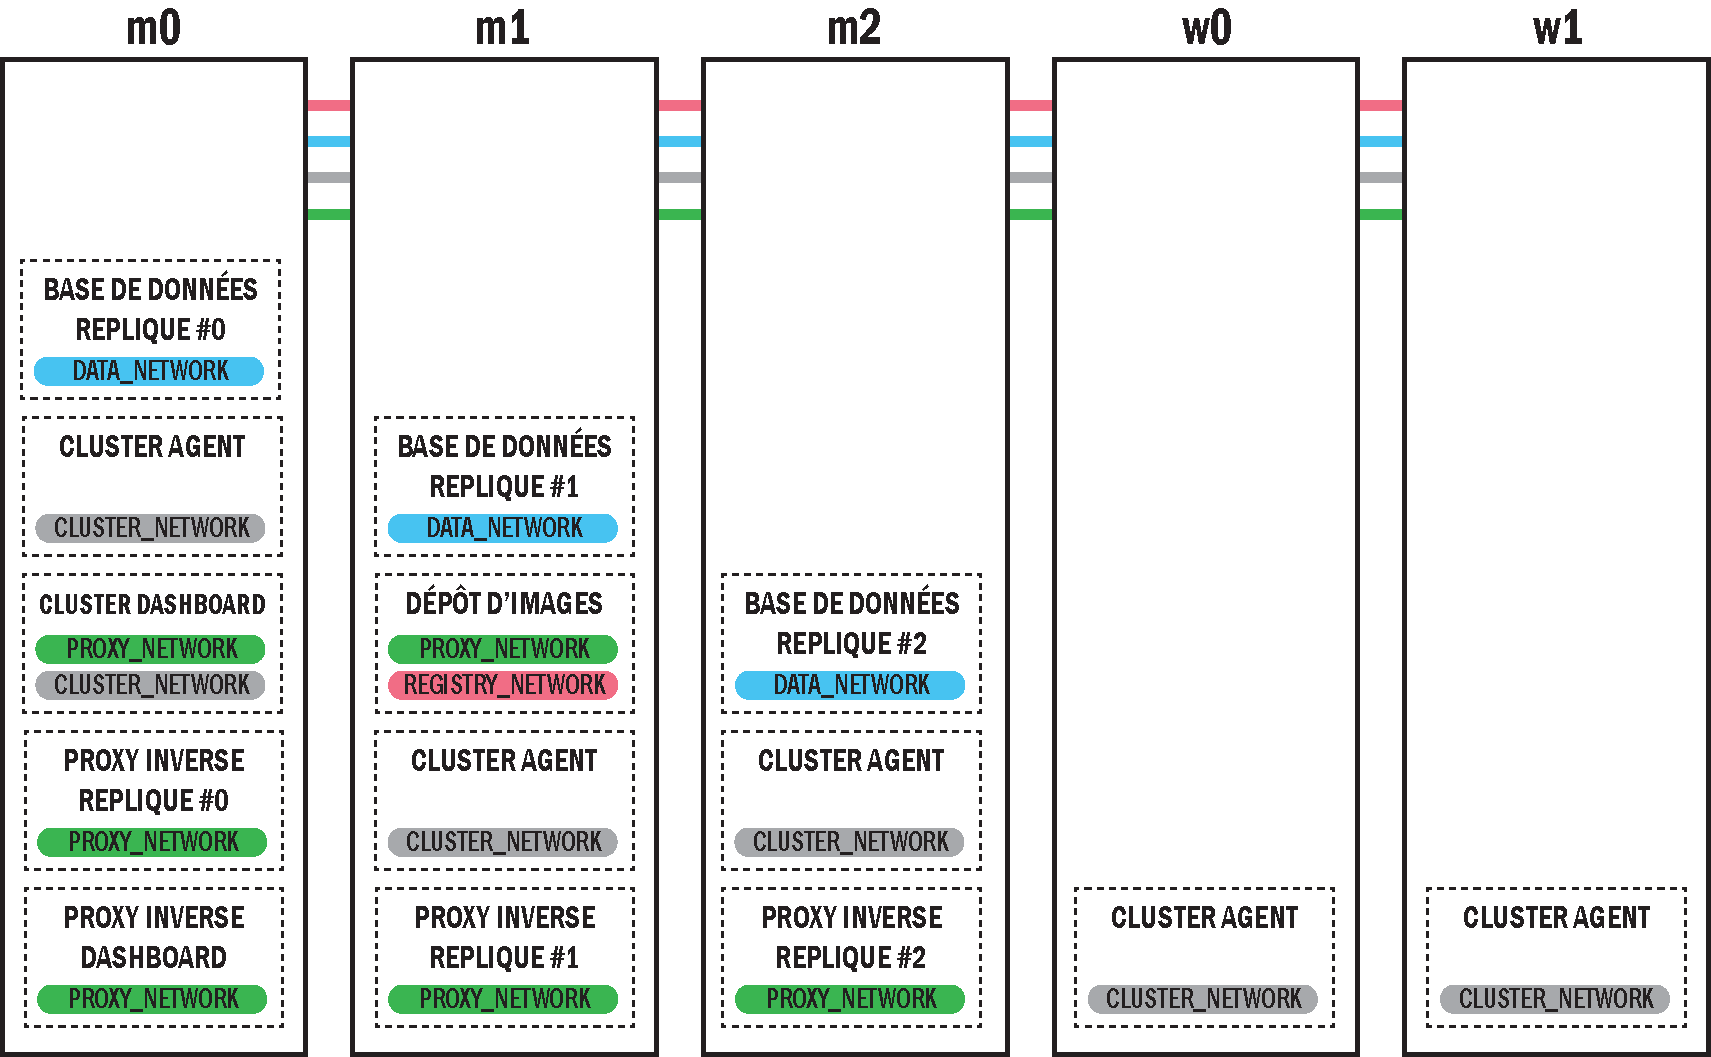
\includegraphics[width=.9\linewidth]{chapter5/containers.pdf}
        \caption{caption}
	\label{fig:containers}
\end{figure}


\section{Experimentations}

\subsection{Installation Matérielle}

\subsection{Haute disponibilité}

\section{Conclusion}